\chapter{Appendix: LSD Layer Analysis}
\label{sec:layers}

In the following, a visual comparison of the LSD output with different numbers of layers is shown. Note that better results were achieved using more layers. This, however, comes at the price of higher computational overhead. A tradeoff must be found to achieve good LSD performance on a limited embedded processor.

\section{2 Layers}

\cref{fig:2_layers} shows the issue of flying with too few layers. At two layers, the coarsest resolution is too detailed for the incoming points at high altitude. Therefore, by the time LSD converges on the SFM information, SFM already exchanges the keyframe which leads to a map movement and therefore the loss of information. Because of this, LSD has a hard time detecting any landing sites.

\begin{figure}[h]
\centering
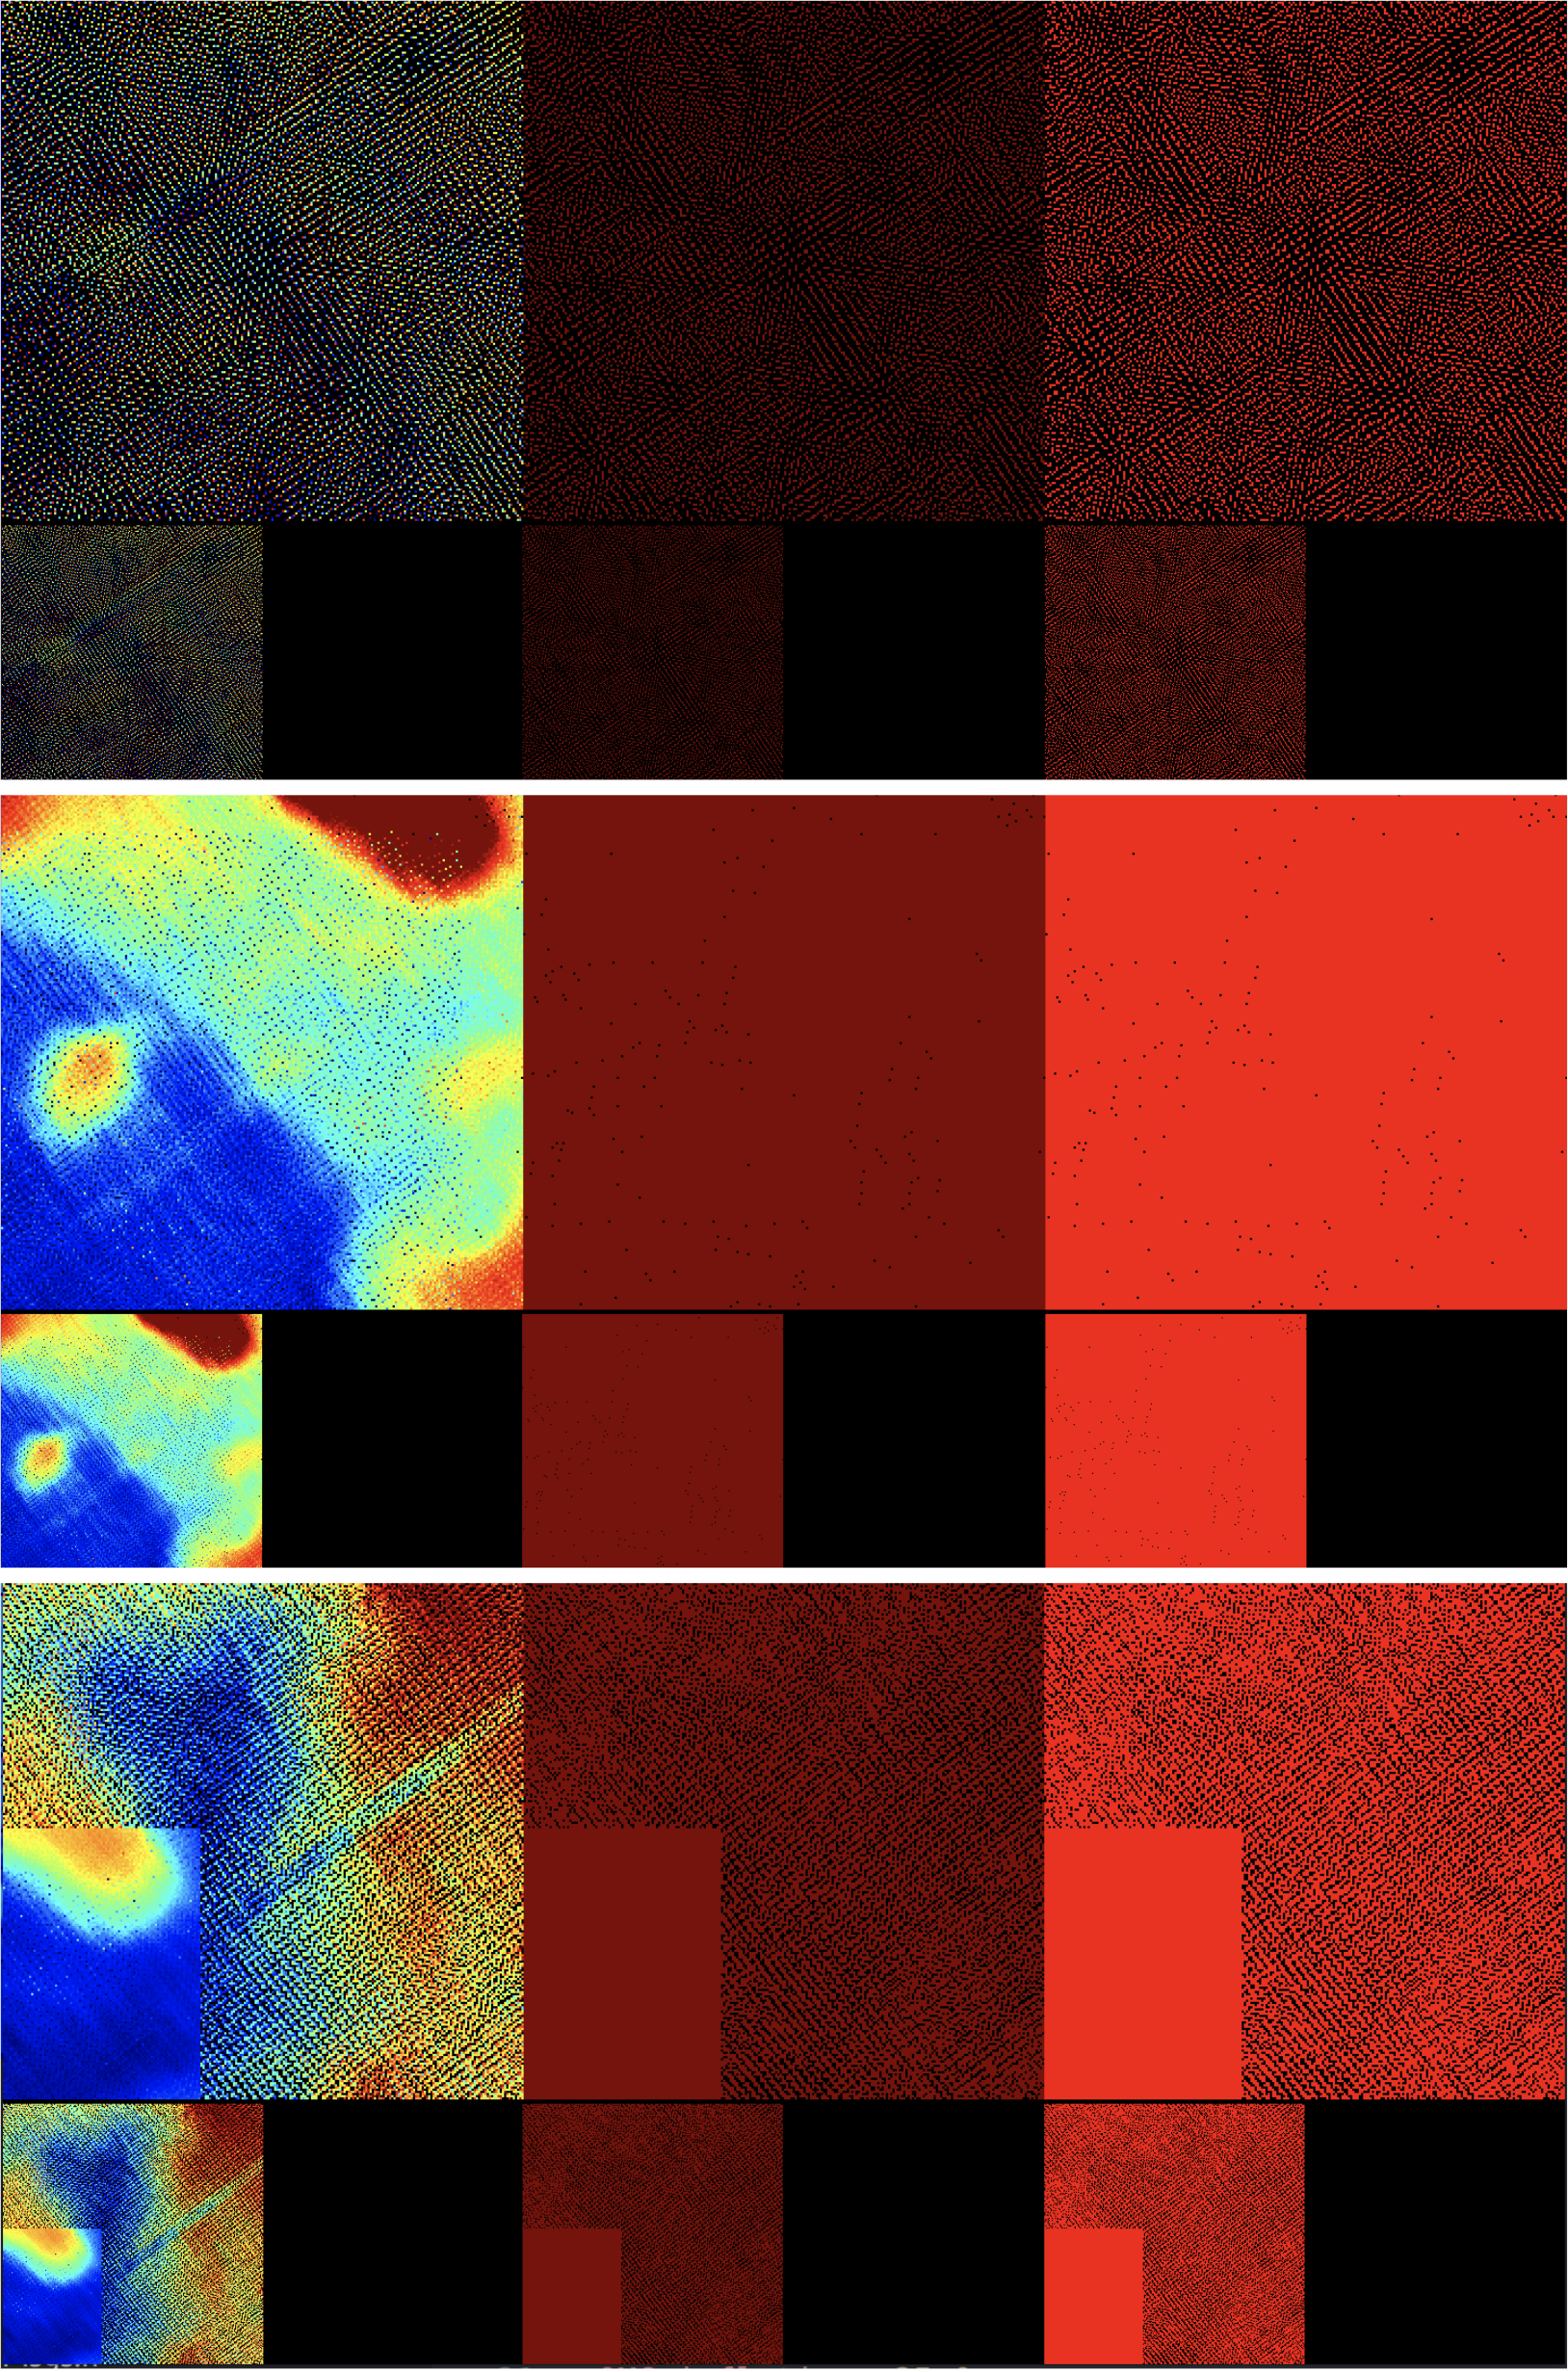
\includegraphics[scale=0.44]{images/appendix/layers/2.png}
\caption{LSD DEM with two layers: The top third shows the map after it received an iteration of sparse inputs from SFM. The middle image shows the map after some conversion time. The bottom third shows the map after the map movement. Note the retained information in the bottom left corner}
\label{fig:2_layers}
\end{figure}

\section{3 Layers}

\cref{fig:3_layers} shows the same chain of events but with 3 layers. Note that the input is less sparse and the DEM is able to detect landing sites before the map is moved.

\begin{figure}[h]
\centering
\includegraphics[scale=0.6]{images/appendix/layers/3.png}
\caption{LSD DEM with three layers: The top third shows the map after it received an iteration of sparse inputs from SFM. The middle image shows the map after some conversion time. The bottom third shows the map after the map movement. Note the retained information in the bottom left corner}
\label{fig:3_layers}
\end{figure}

\section{4 Layers}

Again \cref{fig:4_layers} shows the map updates for 4 layers. With this setting, landing sites were perceived more consistently and much faster.

\begin{figure}[h]
\centering
\includegraphics[scale=0.5]{images/appendix/layers/4.png}
\caption{LSD DEM with four layers: The top third shows the map after it received an iteration from SFM. The middle image shows the map after some conversion time. The bottom third shows the map after the map movement. In this case, the keyframe location difference before and after the movement was so big that the entire DEM was emptied and the LS segmentation doesn't find valid sites again.}
\label{fig:4_layers}
\end{figure}